
Um algoritmo de força bruta consiste na verificação sistemática de todas as possibilidades até que se consiga encontrar a correta para atender determinada condição. No pior caso o algoritmo precisaria percorrer todo o espaço de busca, o que demandaria um grande esforço computacional.

A força bruta para quebra da chave de criptografia consiste basicamente em conhecer o valor $n$ da chave pública e buscar $p$ e $q$ através de sucessivas divisões até que se encontre a operação que resulte em resto 0. Em posse de $p$ e $q$, calcula-se o totiente $\phi(n)$, e em seguida o inverso multiplicativo (via algoritmo de Euclides) para $\phi$ e $e$ da chave pública, encontrando $d$ da chave privada. Dependendo do tamanho da palavra, a busca por $p$ e $q$ pode demandar muito tempo, sendo essa a condição que garante a segurança do RSA.

Para realizar a quebra da chave também é possível se utilizar do algoritmo Pollard-Rho, que possui uma melhor performance nos casos em que a fatoração de grandes números que tenham fatores primos pequenos. A heurística se baseia em um algoritmo de detecção de ciclos para encontrar um dos valores gerados. Mesmo não garantindo tempo de execução, o pior cenário costuma ter complexidade $O(\sqrt{n})$, sendo $n$ o fator modular de $p$ e $q$ \cite{cormen:02}.

Na tabela~\ref{tab:breakTable} abaixo foi realizado um teste comparativo para averiguar a diferença de performance na quebra da chave utilizando de um algoritmo de força bruta (até $\sqrt{n}$) e Pollard-Rho. Para a geração de chave foram utilizados os mesmos algoritmos citados anteriormente e a comparação realizada contemplou todas as combinações de geração (Prime, Miller-Rabin e Fermat) e quebra de chave (Brutal Force e Pollard Rho).

% Please add the following required packages to your document preamble:
% \usepackage{multirow}
\begin{table}[!htbp]
\centering
\caption{Tempo de quebra de chaves (segundos) \textit{x} número de bits.}
\label{tab:breakTable}
\begin{tabular}{|c|l|l|l|l|l|l|}
\hline
\multirow{\textbf{Bits}} & \multicolumn{3}{c|}{\textbf{Brutal Force}} & \multicolumn{3}{c|}{\textbf{Pollard Rho}} \\ \cline{2-7} 
 & \textbf{Prime} & \textbf{Miller} & \textbf{Fermat} & \textbf{Prime} & \textbf{Miller} & \textbf{Fermat} \\ \hline
\textbf{4} & 0.0003 & 0.0002 & 0.0004 & 0.0002 & 0.0002 & 0.0002 \\ \hline
\textbf{8} & 0.0003 & 0.0003 & 0.0005 & 0.0003 & 0.0003 & 0.0003 \\ \hline
\textbf{16} & 0.0075 & 0.0062 & 0.0121 & 0.0061 & 0.0045 & 0.0038 \\ \hline
\textbf{24} & 1.3865 & 1.4948 & 1.4153 & 0.0576 & 0.0638 & 0.0803 \\ \hline
\textbf{32} & 621.03 & 476.90 & 667.88 & 1.1744 & 1.1017 & 1.3571 \\ \hline
\end{tabular}
\end{table}

A Figura~\ref{Fig:bruteforceFig} demonstra os tempos de quebra de chaves \textit{x} número de bits da chave para a implementação do ataque de força bruta proposto neste trabalho, assim como na Figura~\ref{Fig:pollardFig} a quebra de chaves com o algoritmo de \textit{Pollard Rho}. Analisando o gráfico percebe-se que o tempo de execução da função de quebra por força bruta é de complexidade de tempo exponencial em relação à quantidade de bits da entrada, tornando-se computacionalmente inviável a quebra de chaves com valores muito grandes. Contudo, é nítida a diferença de tempo de quebra de chaves via força bruta e Pollard Rho, valendo ressaltar a diferença na escala de tempo dos dois gráficos - Força Bruta de 0 a 600 segundos e Pollard Rho de 0 a 1.4 segundos.

\begin{figure}[!htbp]
   \begin{minipage}{0.48\textwidth}
     \centering
     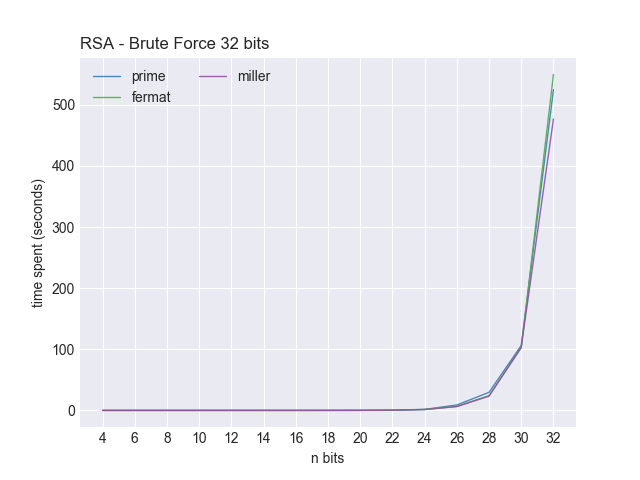
\includegraphics[width=1.1\linewidth]{images/32_BruteForce.png}
     \caption{Força bruta.}\label{Fig:bruteforceFig}
   \end{minipage}\hfill
   \begin{minipage}{0.48\textwidth}
     \centering
     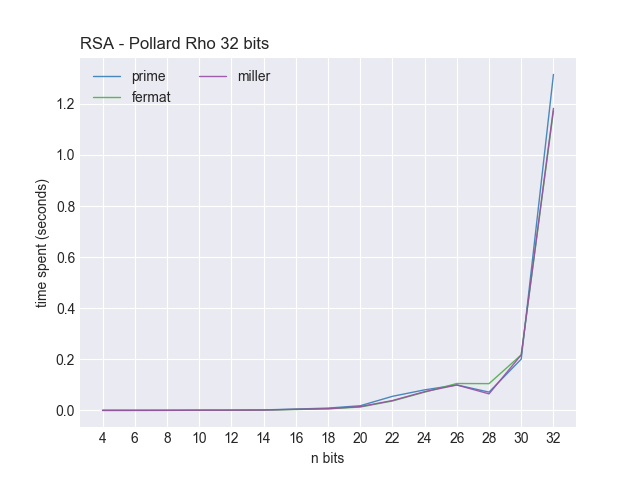
\includegraphics[width=1.1\linewidth]{images/32_PollardRho.png}
     \caption{Pollard Rho.}\label{Fig:pollardFig}
   \end{minipage}
\end{figure}

